% !TEX TS-program = pdflatexmk

\documentclass[12pt,compress]{beamer}
\usepackage{newtxtext,newtxmath}
\usepackage[utf8]{inputenc}
\usepackage{microtype}
\usepackage{array}
\usepackage{hyperref}
\usepackage{graphicx}
\usepackage{setspace}
\usepackage{tikz}
\usetikzlibrary{shapes.multipart}
\usetikzlibrary{positioning}
\usetikzlibrary{arrows}
\usepackage{pgfplots}
\pgfplotsset{compat=1.7}
\usepackage{forest}
\useforestlibrary{linguistics}
\usepackage{appendixnumberbeamer}
\usepackage[style=authoryear,maxbibnames=99,sorting=nyt,backend=biber]{biblatex}
\AtEveryBibitem{\clearfield{note}}


\addbibresource{bethard.bib}
\addbibresource{extra.bib}
\renewcommand*{\bibfont}{\scriptsize}

% Define UA colors
% https://brand.arizona.edu/guide/color
\definecolor{ua-red}{HTML}{AB0520}
\definecolor{ua-blue}{HTML}{0C234B}

\colorlet{event}{ua-red}
\colorlet{time}{ua-blue}
\colorlet{partialtime}{time!50!white}
\tikzset{
  relation-type/.style={auto, font=\scriptsize\scshape},
  relation-path/.style={thick, ->},
  on/.code n args={2}{\alt<#1>{\pgfkeysalso{#2}}{}},
  annotate on/.code n args={2}{\alt<#1>{}{\pgfkeysalso{opacity=0, every #2 node part/.style={text opacity=1}}}},
  relation label/.style={edge node={node[auto, font=\scshape, inner sep=2pt]{#1}}},
  hid/.style 2 args={
    rectangle split,
    rectangle split horizontal,
    draw=#2,
    rectangle split parts=#1,
    fill=#2!40,
    outer sep=1mm},
}
\setlength\fboxrule{1pt}
\setlength\fboxsep{1pt}
\newcommand{\eventbox}[1]{\fcolorbox{event}{white}{#1}}
\newcommand{\timebox}[1]{\fcolorbox{time}{white}{#1}}
\newcommand{\smallcite}[1]{{\scriptsize\parencite{#1}}}
\newcommand{\nonterm}[1]{\textsc{[#1]}}
\newcommand{\word}[1]{\textit{#1}}
\newcommand{\operator}[1]{\textsc{#1}}

% smaller than \strut, but ensures a constant height
\newcommand{\fullheight}{\vphantom{(p}}

% command for annotating words in text
% #1: drawing options
% #2: name of entire shape
% #3: number of parts
% #4: name of baseline part
% #5: annotation type
% #6: node text following \nodepart{two}
\newcommand{\annotate}[6][]{%
\tikz[remember picture,baseline={(#2.#4)}]{%
\node[
  rectangle split,
  rectangle split parts=#3,
  thick,
  inner sep=2pt,
  align=center,
  draw=event,
  #1]%
(#2)
{%
\scriptsize\fullheight\textsc{#5}%
\nodepart{two}%
#6%
\fullheight};}}

% short commands for annotations of various sizes
\newcommand{\AnnotateTwo}[4][]{\annotate[#1]{#2}{2}{two}{#3}{#4}}
\newcommand{\AnnotateThree}[5][]{\annotate[#1]{#2}{3}{three}{#3}{%
\scriptsize\fullheight\textsc{#4}%
\nodepart{three}%
#5}}
\newcommand{\AnnotateFour}[6][]{\annotate[#1]{#2}{4}{four}{#3}{%
\scriptsize\fullheight\textsc{#4}%
\nodepart{three}%
\scriptsize\fullheight\textsc{#5}%
\nodepart{four}%
#6}}
\newcommand{\AnnotateFive}[7][]{\annotate[#1]{#2}{5}{five}{#3}{%
\scriptsize\fullheight\textsc{#4}%
\nodepart{three}%
\scriptsize\fullheight\textsc{#5}%
\nodepart{four}%
\scriptsize\fullheight\textsc{#6}%
\nodepart{five}%
#7}}
\newcommand{\AnnotateSix}[8][]{\annotate[#1]{#2}{6}{six}{#3}{%
\scriptsize\fullheight\textsc{#4}%
\nodepart{three}%
\scriptsize\fullheight\textsc{#5}%
\nodepart{four}%
\scriptsize\fullheight\textsc{#6}%
\nodepart{five}%
\scriptsize\fullheight\textsc{#7}%
\nodepart{six}%
#8}}

% short commands for animated annotations of various sizes
\newcommand{\AnnotateTwoOn}[5][]{\annotate[#1,annotate on={#2}{two}]{#3}{2}{two}{#4}{#5}}

% command for adding links
% #1: drawing options (typically, the color)
% #2: edge options (typically out=NN, in=NN)
% #3: start anchor for arrow
% #4: end anchor for arrow
\newcommand{\AnnotateLink}[4][]{%
\path[color=time,thick,->,#1] (#3) node [circle,color=time,fill,inner sep=0.25ex,#1] {} edge[#2] (#4);}

% command for drawing a timeline
% #1: drawing options
% #2: number of primary intervals
% #3: number of secondary intervals per primary interval
\newcommand{\tikztimeline}[3][]{%
\pgfmathsetmacro{\primaryend}{#2-1}
\pgfmathsetmacro{\secondaryend}{#3-1}
% horizontal line
\draw[#1,dashed] (-0.33,0) -- (0,0);
\draw[#1] (0,0) -- (#2,0);
\draw[#1,dashed,-latex] (#2,0) -- (#2 + 0.33,0);
% primary ticks
\foreach \primary  in {0,...,\primaryend} {%
  \draw[#1] (\primary,0) -- (\primary,\normalbaselineskip);
  % secondary ticks
  \foreach \secondary [evaluate=\secondary] in {\primary+1/#3,\primary+.../#3,\primary+\secondaryend/#3} {
    \draw[#1] (\secondary,0) -- (\secondary,0.5\normalbaselineskip);
  }
}
\draw[#1] (#2,0) -- (#2,\normalbaselineskip);
}

% command for drawing a interval on a timeline
% #1: drawing options
% #2: start time (i.e., start x position)
% #3: end time (i.e., start x position)
% #4: vertical tier (i.e., y position)
% #5: text
\newcommand{\tikztimelineinterval}[5][]{%
\draw[line width=0.9\normalbaselineskip,draw=time,text=white,#1] (#2, #4\normalbaselineskip) -- (#3, #4\normalbaselineskip) node[midway,font=\footnotesize] {#5};
}

% short command for drawing an interval the width of a single primary interval
\newcommand{\tikztimelineprimaryinterval}[4][]{\tikztimelineinterval[#1]{#2}{#2+1}{#3}{#4}}


\mode<presentation>{
\usetheme{Madrid}
\usecolortheme[named=ua-red]{structure}
\setbeamertemplate{navigation symbols}{}
\setbeamertemplate{section in toc}[square]
\setbeamertemplate{subsection in toc}[square]
\setbeamertemplate{items}[square]
\setbeamercovered{invisible}
}

\newcommand{\host}{University of Arizona}
\newcommand{\texttoday}{16 Feb 2019}
\newcommand{\isotoday}{2019-02-16}
\newcommand{\isodaybeforeyesterday}{2019-02-14}
\newcommand{\isoweekofmarchsix}{2019-W10}

\title[\url{http://bethard.faculty.arizona.edu/}]{Human annotation and machine learning in understanding the language of time}
\author{Dr. Steven Bethard}
\institute[University of Arizona]{%
School of Information\\
University of Arizona}
\date{\texttoday}

\begin{document}


\section{Motivation: inferring timelines is challenging for computers}


\begin{frame}[plain]
  \titlepage
\end{frame}


\begin{frame}{An interactive timeline of the 2011 Arab Spring}
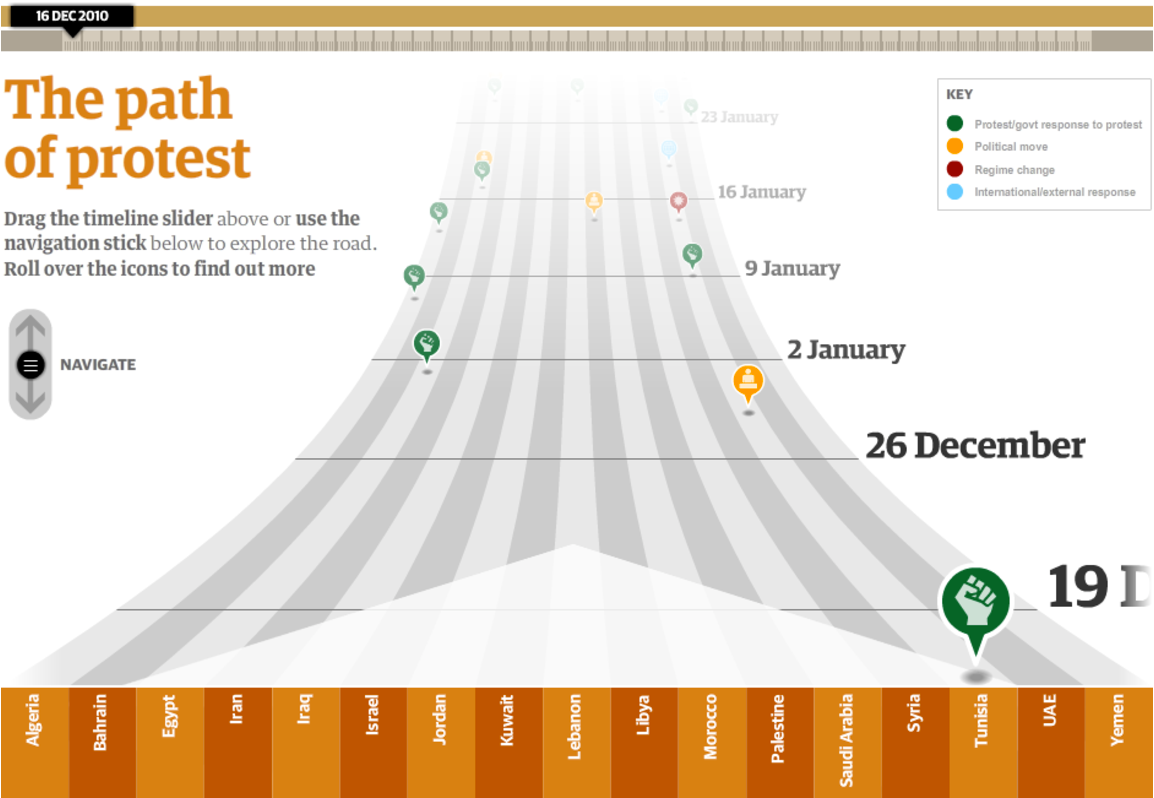
\includegraphics[width=0.9\textwidth]{arab-spring}

\tiny
Source: \url{http://www.guardian.co.uk/world/interactive/2011/mar/22/middle-east-protest-interactive-timeline}
\end{frame}


\begin{frame}{An interactive patient timeline}
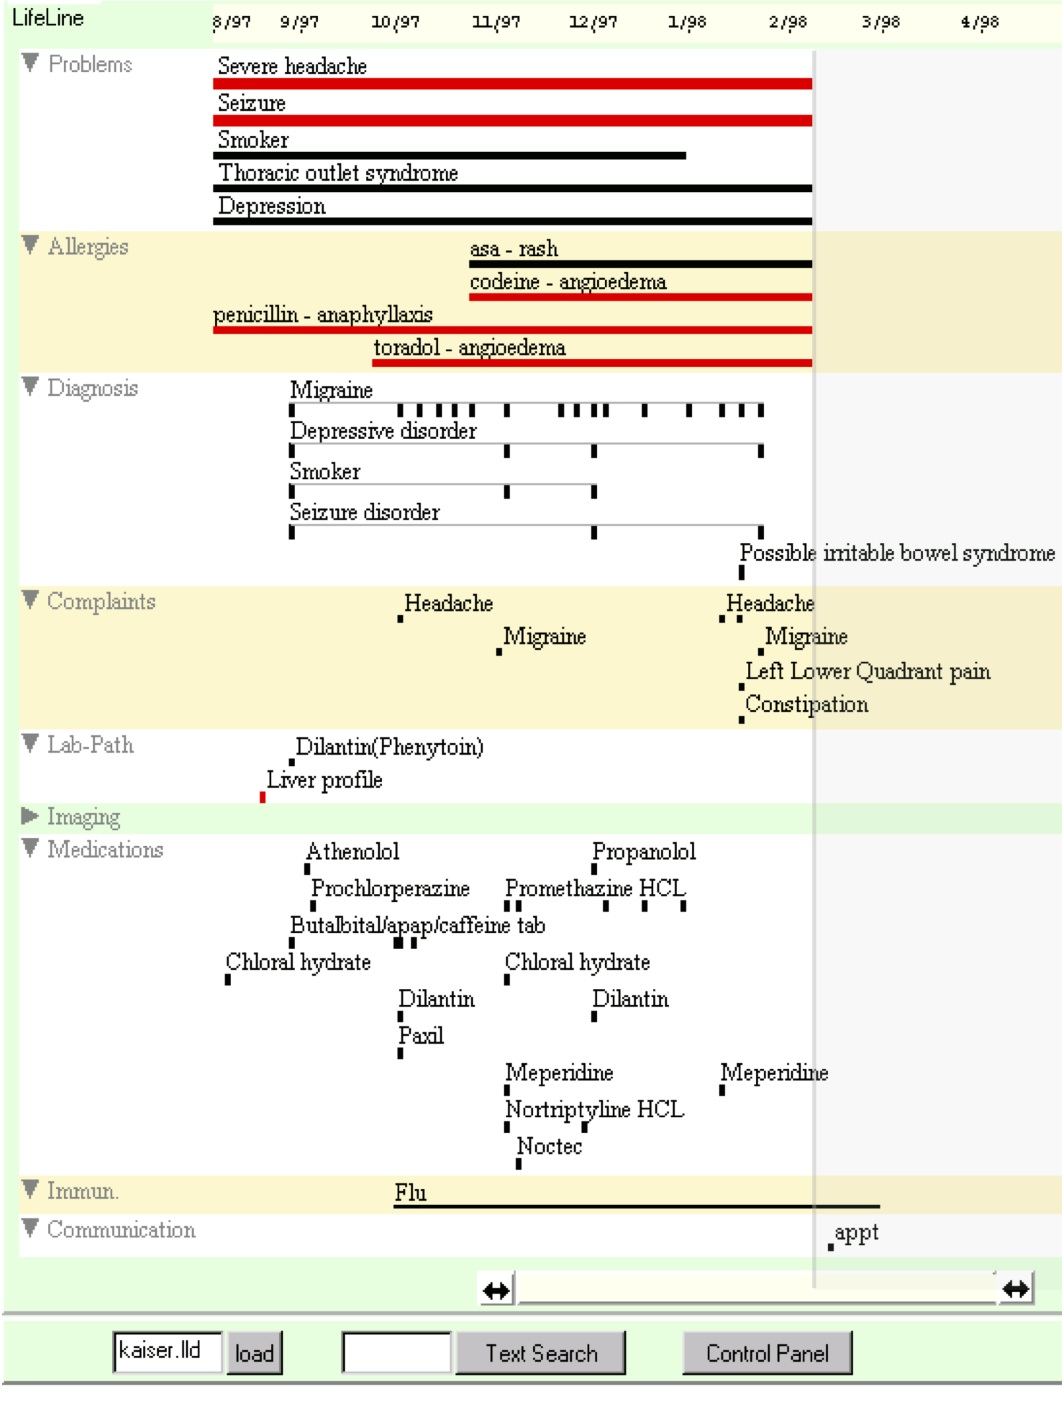
\includegraphics[width=\textwidth,trim={0 5.1in 0 0},clip]{kaiserlifelines.jpg}

\tiny
Source: \url{http://www.cs.umd.edu/hcil/lifelines/}
\end{frame}


\begin{frame}{A timeline model should predict like humans}
\begin{tikzpicture}[auto]
\node (text) {\parbox{0.225\textwidth}{\tiny At least 11 people have died in new clashes with security forces in Tunisia after four weeks of unrest, it was reported today.
Rioting against joblessness and other social ills has scarred many cities in the country since 17 December, when a 26-year-old graduate set himself on fire\ldots}};
\node (human) [right=2em of text] {
  \begin{tikzpicture}[auto]
  \node at (0, 1) (1) {
\includegraphics[width=0.2\textwidth]{male-user}};
  \node at (0.5, 0.5) (2) {
\includegraphics[width=0.2\textwidth]{female-user}};
  \end{tikzpicture}
  }
  edge [<-,ultra thick] (text);
\node (model) [right=2em of text,below=of human] {$\text{\LARGE h}\left(\text{\parbox{0.225\textwidth}{\tiny
At least 11 people have died in new clashes with security forces in Tunisia after four weeks of unrest, it was reported today.
Rioting against joblessness and other social ills has scarred many cities in the country since 17 December, when a 26-year-old graduate set himself on fire\ldots
}}\right)$}
  edge [<-,ultra thick] (text);
\node (timeline) [right=2em of human,right=of model] {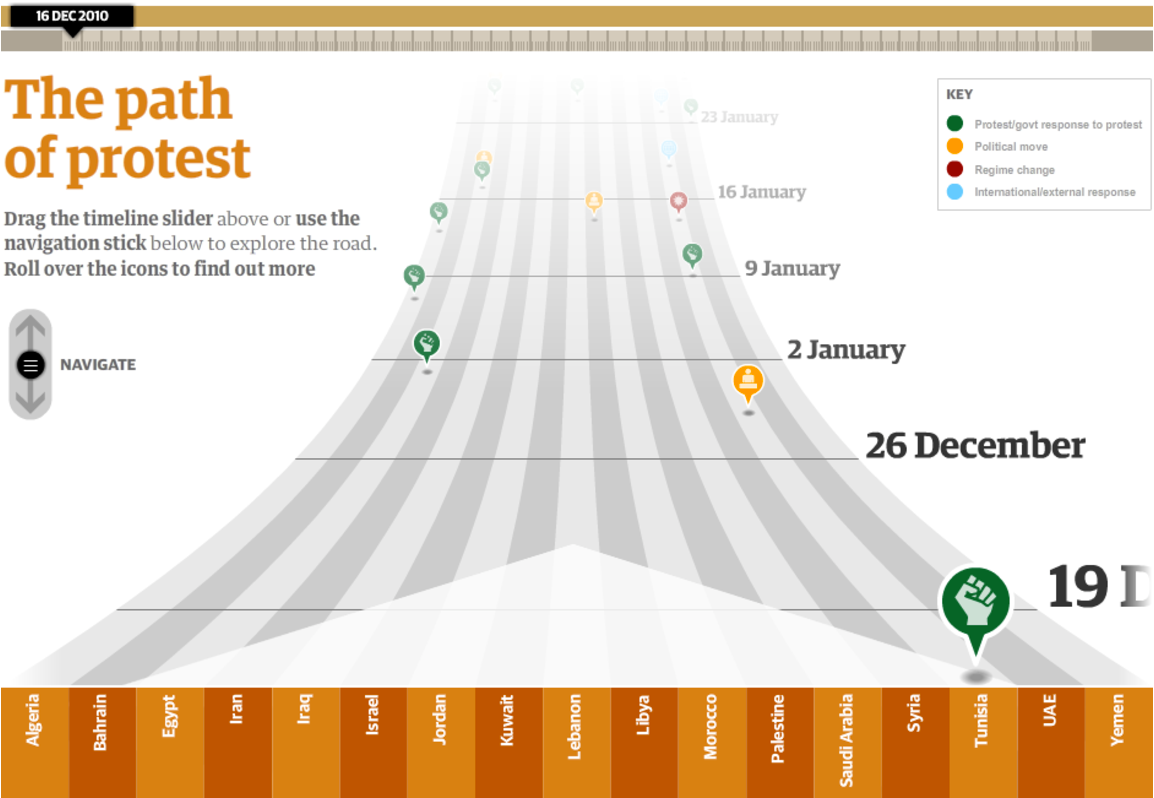
\includegraphics[width=0.25\textwidth]{arab-spring}}
  edge [<-,ultra thick]  (human)
  edge [<-,ultra thick]  (model);
\end{tikzpicture}

\vfill
\tiny Sample text from \url{https://www.theguardian.com/world/2011/jan/09/tunisia-clashes-weeks-unrest}
\end{frame}


\begin{frame}{Open issues in training a timeline model}
\begin{itemize}
\item Translating directly from text to visualization is infeasible
\begin{itemize}
\item What are appropriate intermediate representations?
\end{itemize}
\bigskip
\item Human annotation is needed to provide training examples
\begin{itemize}
\item How do we reliably elicit human understanding of timelines?
\end{itemize}
\bigskip
\item Intermediate representations must be (machine) learnable
\begin{itemize}
\item How best can we frame subtasks as machine learning problems?
\end{itemize}
\end{itemize}
\end{frame}


\begin{frame}{ISO-TimeML represents timelines as graphs}{\smallcite{pustejovsky2003timeml,pustejovsky2010iso}}
\begin{columns}
\begin{column}{0.35\textwidth}
\small
At least 11 people have died in new clashes with security forces in Tunisia after four weeks of unrest, it was reported today.
Rioting against joblessness and other social ills has scarred many cities in the country since 17 December, when a 26-year-old graduate set himself on fire when police confiscated his fruits and vegetables for selling without a permit\ldots
\end{column}
{\Huge $\Rightarrow$}
\begin{column}{0.55\textwidth}
\small
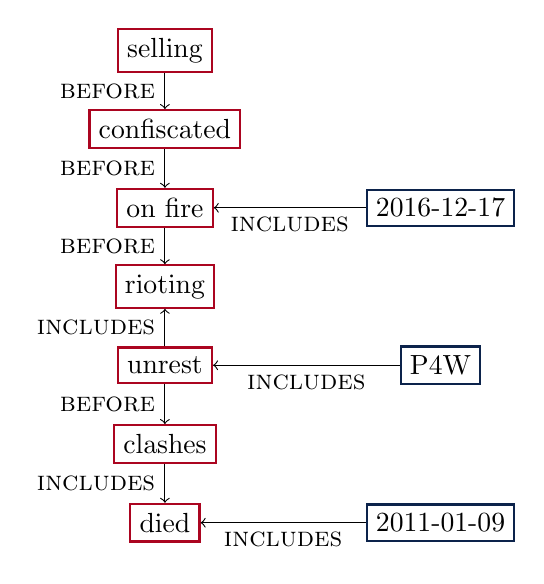
\begin{tikzpicture}[auto]
\node[draw=event,thick] at (0, 6) (selling) {selling};
\node[draw=event,thick] at (0, 5) (confiscated) {confiscated}
  edge [<-] node {\textsc{before}} (selling);
\node[draw=event,thick] at (0, 4) (on fire) {on fire}
  edge [<-] node {\textsc{before}} (confiscated);
\node[draw=time,thick] at (3.5, 4) (17 December) {2016-12-17}
  edge [->] node {\textsc{includes}} (on fire);
\node[draw=event,thick] at (0, 3) (rioting) {rioting}
  edge [<-] node {\textsc{before}} (on fire);
\node[draw=event,thick] at (0, 2) (unrest) {unrest}
  edge [->] node {\textsc{includes}} (rioting);
\node[draw=time,thick] at (3.5, 2) (four weeks) {P4W}
  edge [->] node {\textsc{includes}} (unrest);
\node[draw=event,thick] at (0, 1) (clashes) {clashes}
  edge [<-] node {\textsc{before}} (unrest);
\node[draw=event,thick] at (0, 0) (died) {died}
  edge [<-] node {\textsc{includes}} (clashes);
\node[draw=time,thick] at (3.5, 0) (today) {2011-01-09}
  edge [->] node {\textsc{includes}} (died);
\end{tikzpicture}
\end{column}
\end{columns}
\end{frame}


\begin{frame}{Outline}
\tableofcontents
\end{frame}


\AtBeginSection[]
{
 \begin{frame}<beamer>
 \frametitle{Outline}
 \tableofcontents[currentsection]
 \end{frame}
}


\section{Temporal relations: annotations and models often co-evolve}


\begin{frame}{Where should we annotate temporal relations?}
\strut\alert{
\only<2-4>{TimeBank \smallcite{pustejovsky2003timebank}: salience}%
\only<5-7>{TempEval \smallcite{verhagen-EtAl:2010:SemEval}: frequent pairs}%
\only<8-10>{Dense Timebank \smallcite{cassidy-etal:2014:ACLShort}: all nearby pairs}%
}

\strut\alert{
\only<4,7,10>{Human agreement:}
\only<4>{0.55}%
\only<7>{0.65}%
\only<10>{0.65}%
}

\strut\alert{
\only<4,7,10>{Model performance:}
\only<4>{\textasciitilde 0.60 accuracy}%
\only<7>{\textasciitilde 0.60 accuracy}%
\only<10>{\textasciitilde 0.50 F1}%
}

``There were four or five people inside, and they just
\AnnotateTwo{started}{event}{started}
\AnnotateTwo{firing}{event}{firing}.''
\\[1.25\baselineskip]
Ms. Sanders was
\AnnotateTwo{hit}{event}{hit} several times and was
\AnnotateTwo{pronounced}{event}{pronounced}
\AnnotateTwo{dead}{event}{dead}
at
\\[1.25\baselineskip]
the scene. The other customers
\AnnotateTwo{fled}{event}{fled},
and the police
\AnnotateTwo{said}{event}{said}
it did not
\\[1.25\baselineskip]
\AnnotateTwo{appear}{event}{appear}
that anyone else was
\AnnotateTwo{injured}{event}{injured}.
\begin{tikzpicture}[remember picture, overlay]
\only<3-4>{
\AnnotateLink{out=60, in=210, relation label=after, pos=0.05}{fled.north}{started.south}
\AnnotateLink{out=20, in=200, relation label=is-included}{hit.north}{firing.south}
\AnnotateLink{out=165, in=15, relation label=after, swap}{pronounced.west}{hit.east}
}
\only<6-7>{
\AnnotateLink{out=15, in=165, relation label=overlap-or-after}{appear.east}{injured.west}
\AnnotateLink{out=315, in=135, relation label=overlap}{hit.south}{fled.north}
\AnnotateLink{out=210, in=30, relation label=before}{started.south}{hit.north}
}
\only<9->{
\AnnotateLink{}{started.south}{firing}
\AnnotateLink{}{started.south}{firing}
\AnnotateLink{}{started.south}{hit}
\AnnotateLink{}{started.south}{pronounced}
\AnnotateLink{}{started.south}{dead}
\AnnotateLink{}{hit.east}{firing}
\AnnotateLink{}{firing.south}{pronounced}
\AnnotateLink{}{firing.south}{dead}
\AnnotateLink{}{hit.east}{pronounced}
\AnnotateLink{}{hit.east}{dead}
\AnnotateLink{}{hit.east}{said}
\AnnotateLink{}{dead.south}{pronounced}
\AnnotateLink{}{fled.east}{pronounced}
\AnnotateLink{}{pronounced.south}{said}
\AnnotateLink{}{dead.south}{said}
\AnnotateLink{}{fled.east}{said}
\AnnotateLink{}{fled.south}{appear}
\AnnotateLink{}{appear.east}{said}
\AnnotateLink{}{injured.east}{said}
\AnnotateLink{}{injured.west}{appear}
}
\end{tikzpicture}
%NYT19980212.0019
%TBE TBEI  TE2
%e20 ei226 e19 started
%e50 ei227 e20 firing
%e21 ei228 e21 hit
%e22 ei229 e22 pronounced
%e51 ei230 e23 dead
%e25 ei231 e24 fled
%e26 ei232 e25 said
%e27 ei233 e26 appear
%e29 ei234 e27 injured
%
%TimeBank:
%fled AFTER started
%hit IS_INCLUDED firing
%pronounced AFTER hit
%
%TempEval 2013:
%fled AFTER started
%hit IS_INCLUDED firing
%pronounced AFTER hit
%
%TempEval 2010:
%appear OVERLAP-OR-AFTER injured
%hit OVERLAP fled
%started BEFORE hit
\end{frame}


\begin{frame}{Decomposing tasks helps humans and machines}
\strut\alert{%
\only<1>{TempEval/Dense TimeBank: arbitrary pairs}%
\only<2->{\cite{bethard-etal:2007:IJSC}: linguistically plausible pairs}}

\strut\alert{\only<6->{Human agreement: 0.90}}

\strut\alert{\only<6->{Model performance: 0.89}}

\smallskip
\AnnotateTwoOn{2-}{turning}{event}{Turning}
its back on
\AnnotateTwo[draw=time]{210-years}{time}{210 years}
of loyalty to the British royal family,
\\
a constitutional convention
\AnnotateTwoOn{2-}{voted}{event}{voted}
overwhelmingly
\AnnotateTwoOn[draw=time]{2-}{friday}{time}{Friday}
to
\AnnotateTwo{make}{Event}{make}\ldots
\begin{tikzpicture}[remember picture,overlay]
\only<1>{
\AnnotateLink{relation label=before}{210-years.south east}{make.west}
}
\end{tikzpicture}

\onslide<3->
\centering
\begin{forest}
for tree={l sep=0.3em, l=0.3em}
[S
  [VP
    [{\eventbox{Turning}},name=turning]
    [{\ldots}]
    [PP
      [on]
      [NP
        [{\timebox{210 years}},name=210years]
        [{\ldots}] ] ] ]
  [{\ldots}]
  [VP
    [{\eventbox{voted}},name=voted]
    [{\ldots}]
    [{\timebox{Friday}},name=friday]
    [VP
      [to]
      [{\eventbox{make}},name=make]
      [{\ldots}] ] ] ]
\only<4>{%
\draw [auto,->] (turning) to [bend right] node [swap] {\textsc{after}} (210years);
\draw [auto,<->] (turning) to [bend left] node [swap] {\textsc{identity}} (voted);
\draw [below,->] (friday) to [bend left] node {\textsc{includes}} (voted);}
\visible<4->{%
\draw [auto,->] (make) to [bend left] node {\textsc{after}} (voted);}
\end{forest}
\end{frame}


\section{Times: annotation schemes can be designed for machine-learning}


\begin{frame}{ISO-TimeML annotates flat time expressions}
\alert{%
ISO-TimeML \smallcite{pustejovsky2010iso}
\hfill
\only<2->{Agreement: 0.75}}
\bigskip

Each flat expression associated with a (partial) date:

%APW19980322.0749
\ttfamily\small
\bigskip
\ldots supposed to conclude by \\
\textless TIMEX3 value="1998-05"\textgreater May\textless/TIMEX3\textgreater

\bigskip
\ldots invited to rejoin \\
\textless TIMEX3 value="1998-03-08"\textgreater two weeks ago\textless/TIMEX3\textgreater

\bigskip
\ldots in Northern Ireland for \\
\textless TIMEX3 value="XXXX-SU"\textgreater the past three summers\textless/TIMEX3\textgreater
\end{frame}


\begin{frame}{Flat time expressions miss important structure}
Problem: ISO-TimeML can't represent times that:
\begin{itemize}
\item don't align to exactly 1 calendar unit, e.g., \textit{the past 2 summers}
\item are relative to events, e.g., \textit{5 days postop}
\item are unions of other times, e.g, \textit{Mondays and Fridays}
\end{itemize}
\pause
\bigskip
Humans understand such times:\\[0.5\baselineskip]
\begin{tabular}{ c c c }
\visible<3->{\it the past 2 summers} &
\visible<7->{\it 5 days postop} &
\visible<11->{\it Mondays and Fridays} \\
\visible<4->{%
\begin{tikzpicture}
\tikztimeline{3}{12}
\only<5->{%
\tikztimelineinterval[draw=event]{3+30/365}{3+40/365}{2}{}} % more than 1/365 just so it's visible
\only<6->{%
\tikztimelineinterval{1+5/12}{1+8/12}{2}{}
\tikztimelineinterval{2+5/12}{2+8/12}{2}{}}
\end{tikzpicture}}
&
\visible<8->{%
\begin{tikzpicture}
\tikztimeline{2}{7}
\only<9->{%
\tikztimelineinterval[draw=event]{6/7}{7/7}{2}{}}
\only<10->{%
\tikztimelineinterval{11/7}{12/7}{2}{}}
\end{tikzpicture}}
&
\visible<12->{%
\begin{tikzpicture}
\tikztimeline{3}{7}
\tikztimelineinterval[draw=white]{0}{0}{4}{}% to ensure full vertical space when others are not shown
\only<13->{%
\tikztimelineinterval[draw=partialtime]{0+1/7}{0+2/7}{4}{}
\tikztimelineinterval[draw=partialtime]{1+1/7}{1+2/7}{4}{}
\tikztimelineinterval[draw=partialtime]{2+1/7}{2+2/7}{4}{}}
\only<14->{%
\tikztimelineinterval[draw=partialtime]{0+5/7}{0+6/7}{3}{}
\tikztimelineinterval[draw=partialtime]{1+5/7}{1+6/7}{3}{}
\tikztimelineinterval[draw=partialtime]{2+5/7}{2+6/7}{3}{}}
\only<15>{%
\tikztimelineinterval{0+1/7}{0+2/7}{2}{}
\tikztimelineinterval{0+5/7}{0+6/7}{2}{}
\tikztimelineinterval{1+1/7}{1+2/7}{2}{}
\tikztimelineinterval{1+5/7}{1+6/7}{2}{}
\tikztimelineinterval{2+1/7}{2+2/7}{2}{}
\tikztimelineinterval{2+5/7}{2+6/7}{2}{}}
\end{tikzpicture}}
\end{tabular}
\end{frame}


\begin{frame}{Flat time expressions are hard for machines}
All the best systems for time normalization from flat time expressions rely on hand-constructed grammars
\smallcite{StroetgenGertz2013:LREjournal,bethard:2013:EMNLP,lee-EtAl:2014:P14-1}

\bigskip
E.g., HeidelTime:
\texttt{\scriptsize%
\begin{itemize}
\item[] \ldots
\item[] {[Tt]oday} $\Rightarrow$ UNDEF-this-day
\item[] {[Tt]he} day after tomorrow $\Rightarrow$ UNDEF-this-day-PLUS-2
\item[] (the|that) weekend $\Rightarrow$ "UNDEF-last-week-WE"
\item[] {[Aa]} year (ago|earlier) $\Rightarrow$ UNDEF-REFUNIT-year-MINUS-1
\item[] \%reMonthNumber/\%reDayNumber/\%reYear4Digit \\
\qquad $\Rightarrow$ group(3)-\%normMonth(group(1))-\%normDay(group(2))
\item[] \ldots
\end{itemize}
}

\bigskip
No machine learning model performed as well as these 10,000+ rules
\end{frame}


\begin{frame}{Compositional times are more expressive}
\alert{SCATE \smallcite{bethard-etal:2016:LREC} \hfill \only<2->{Human agreement: 0.82}}

\bigskip
Annotate formally-defined, semantically-compositional time operators:

\bigskip
\AnnotateThree[draw=time]{ex-mafnj-mondays}{Day-Of-Week}{Type=Monday}{Mondays}
\hspace{0.5em}
\AnnotateFour[draw=time]{ex-mafnj-intersection}{Intersection}{Intervals}{R-Intervals}{%
\\[\baselineskip]
\AnnotateThree[draw=time]{ex-mafnj-and}{Union}{R-Intervals}{and}}
\hspace{0.5em}
\AnnotateThree[draw=time]{ex-mafnj-fridays}{Day-Of-Week}{Type=Friday}{Fridays}
\hspace{0.5em}
\AnnotateFour[draw=time]{ex-mafnj-next}{Next}{Interval=DocTime}{R-Interval}{next}
\hspace{0.5em}
\AnnotateThree[draw=time]{ex-mafnj-january}{Month-Of-Year}{Type=January}{January}
\begin{tikzpicture}[remember picture,overlay]%
\AnnotateLink{out=0, in=120}{ex-mafnj-intersection.two east}{ex-mafnj-next.north}
\AnnotateLink{out=270, in=90}{ex-mafnj-intersection.three split}{ex-mafnj-and.north}
\AnnotateLink{out=90, in=60}{ex-mafnj-and.two west}{ex-mafnj-mondays.north}
\AnnotateLink{out=90, in=120}{ex-mafnj-and.two east}{ex-mafnj-fridays.north}
\AnnotateLink{out=90, in=120}{ex-mafnj-next.three east}{ex-mafnj-january.north}
\end{tikzpicture}
\end{frame}


\begin{frame}[t]{Compositional times enable machine learning}
\alert{\cite{laparra-etal:2018:TACL}}
\bigskip

Step 1: Neural networks learn to find times in text

\smallskip
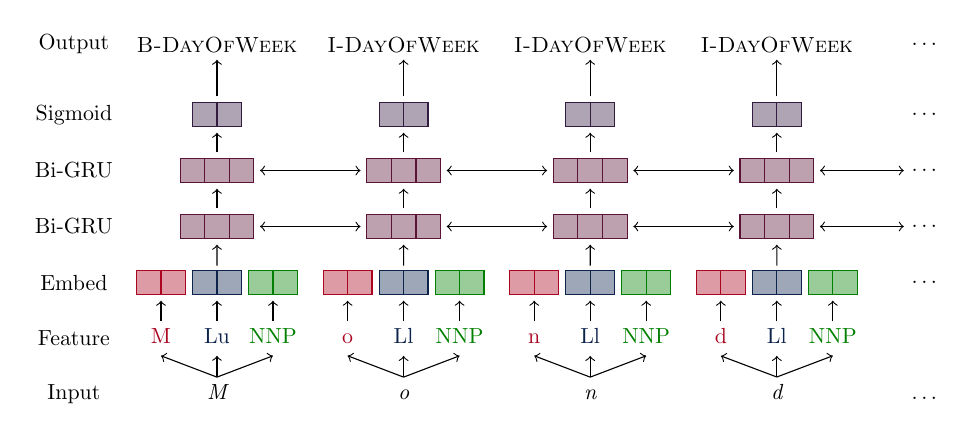
\begin{tikzpicture}[
  scale=0.79, every node/.style={scale=0.79},
  brace/.style={draw,thick,decoration=brace,decorate}]
  \pgfmathsetmacro{\width}{3}
  \pgfmathsetmacro{\height}{0.9}

  \node (1s-i0) at (0.7, 0*\height) {Input};
  \node (1s-fv0) at (0.7, 1*\height) {Feature};
  \node (1s-cv0) at (0.7, 2*\height) {Embed};
  \node (1s-g10) at (0.7, 3*\height) {Bi-GRU};
  \node (1s-g20) at (0.7, 4*\height) {Bi-GRU};
  \node (1s-s0) at (0.7, 5*\height) {Sigmoid};
  \node (1s-o0) at (0.7, 6.25*\height) {Output};

\foreach \c/\f/\g/\h/\o [count=\step from 1] in {M/M/Lu/NNP/{B-DayOfWeek},o/o/Ll/NNP/{I-DayOfWeek},n/n/Ll/NNP/{I-DayOfWeek},d/d/Ll/NNP/{I-DayOfWeek},\ldots} {
    % input character
    \ifdefstring{\c}{\ldots}{
      \node (1s-i\step) at (\step*\width-0.2*\width, 0*\height) {\vphantom{My}\c};
      \node (1s-fv\step) at (\step*\width-0.2*\width, 2*\height) {\ldots};
      \node (1s-g1\step) at (\step*\width-0.2*\width, 3*\height) {\ldots};
      \node (1s-g2\step) at (\step*\width-0.2*\width, 4*\height) {\ldots};
      \node (1s-s\step) at (\step*\width-0.2*\width, 5*\height) {\ldots};
      \node (1s-o\step) at (\step*\width-0.2*\width, 6.25*\height) {\ldots};
    }{
      \node[font=\itshape] (1s-i\step) at (\step*\width, 0*\height) {\vphantom{My}\c};
      \node[text={ua-red}] (1s-f1\step) at (\step*\width-0.3*\width, 1*\height) {\vphantom{My}\f};
      \node[text={ua-blue}] (1s-f2\step) at (\step*\width, 1*\height) {\vphantom{My}\g};
      \node[text={green!50!black}] (1s-f3\step) at (\step*\width+0.3*\width, 1*\height) {\vphantom{My}\h};
      \node[hid={2}{ua-red}] (1s-fv1\step) at (\step*\width-0.3*\width, 2*\height) {};
      \node[hid={2}{ua-blue}] (1s-fv2\step) at (\step*\width, 2*\height) {};
      \node[hid={2}{green!50!black}] (1s-fv3\step) at (\step*\width+0.3*\width, 2*\height) {};
      \node[hid={3}{ua-red!50!ua-blue}] (1s-g1\step) at (\step*\width, 3*\height) {};
      \node[hid={3}{ua-red!50!ua-blue}] (1s-g2\step) at (\step*\width, 4*\height) {};
      \node[hid={2}{ua-red!25!ua-blue}] (1s-s\step) at (\step*\width, 5*\height) {};
      \node[align=center,font=\scshape] (1s-o\step) at (\step*\width, 6.25*\height) {\o};
      \draw[->] (1s-i\step.north) -> (1s-f1\step.south);
      \draw[->] (1s-i\step.north) -> (1s-f2\step.south);
      \draw[->] (1s-i\step.north) -> (1s-f3\step.south);
      \draw[->] (1s-f1\step.north) -> (1s-fv1\step.south);
      \draw[->] (1s-f2\step.north) -> (1s-fv2\step.south);
      \draw[->] (1s-f3\step.north) -> (1s-fv3\step.south);
      \draw[->] (\step*\width, 2.3*\height) -> (1s-g1\step.south);
      \draw[->] (1s-g1\step.north) -> (1s-g2\step.south);
      \draw[->] (1s-g2\step.north) -> (1s-s\step.south);
      \draw[->] (1s-s\step.north) -> (1s-o\step.south);
    }
    % recurrent links
    \ifdefstring{\step}{1}{}{
      \pgfmathtruncatemacro{\last}{add(\step,-1)}
      \draw[<->] (1s-g1\last.east) -> (1s-g1\step.west);
      \draw[<->] (1s-g2\last.east) -> (1s-g2\step.west);
    }
  }
\end{tikzpicture}
\end{frame}


\begin{frame}[t]{Compositional times enable machine learning}
\alert{\cite{laparra-etal:2018:TACL}}

\bigskip
Step 2: Schema-driven heuristic composes nearby identified operators

\smallskip
$\operatorname{Intersection}(\operatorname{Union}(Mondays, Fridays), \operatorname{Next}(\operatorname{DocTime}, January))$

\pause
\bigskip
Step 3: Temporal logic composes operators to yield timeline intervals:

\smallskip
$\vphantom{\left(\text{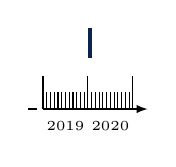
\begin{tikzpicture}[xscale=0.57, baseline={(current bounding box.center)}]
\tikztimeline{2}{12}
\tikztimelineinterval{1+0/12}{1+1/12}{2}{}
\tikztimelineinterval[draw=none,text=black]{0}{1}{-0.5}{\tiny 2019}
\tikztimelineinterval[draw=none,text=black]{1}{2}{-0.5}{\tiny 2020}
\end{tikzpicture}}\right)}
\alt<6->%
% Intersection(Union(Mondays, Fridays), Next(DocTime, January)) as timeline
{\text{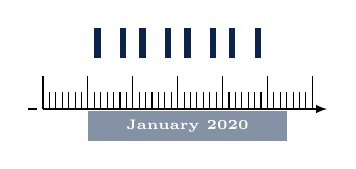
\begin{tikzpicture}[xscale=0.57, baseline={(current bounding box.center)}]
\tikztimeline{6}{7}
\tikztimelineinterval{1+1/7}{1+2/7}{2}{}
\tikztimelineinterval{1+5/7}{1+6/7}{2}{}
\tikztimelineinterval{2+1/7}{2+2/7}{2}{}
\tikztimelineinterval{2+5/7}{2+6/7}{2}{}
\tikztimelineinterval{3+1/7}{3+2/7}{2}{}
\tikztimelineinterval{3+5/7}{3+6/7}{2}{}
\tikztimelineinterval{4+1/7}{4+2/7}{2}{}
\tikztimelineinterval{4+5/7}{4+6/7}{2}{}
\tikztimelineinterval[draw=partialtime,text=white]{1+0/7}{5+3/7}{-0.5}{\tiny\textbf{January 2020}}
\end{tikzpicture}}}
{\alt<2->%
% Intersection(Union(Mondays, Fridays), Next(DocTime, January)) as operators
{\operatorname{Intersection}\left(
\alt<4->%
% Union(Mondays, Fridays) as timeline
{\text{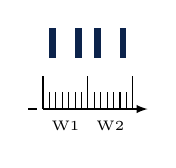
\begin{tikzpicture}[xscale=0.57, baseline={(current bounding box.center)}]
\tikztimeline{2}{7}
\tikztimelineinterval{0+1/7}{0+2/7}{2}{}
\tikztimelineinterval{0+5/7}{0+6/7}{2}{}
\tikztimelineinterval{1+1/7}{1+2/7}{2}{}
\tikztimelineinterval{1+5/7}{1+6/7}{2}{}
\tikztimelineinterval[draw=none,text=black]{0}{1}{-0.5}{\tiny W1}
\tikztimelineinterval[draw=none,text=black]{1}{2}{-0.5}{\tiny W2}
\end{tikzpicture}}}
% Union(Mondays, Fridays) as operator
{\operatorname{Union}\left(
\alt<3->%
% Mondays as timeline
{\text{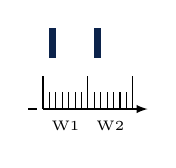
\begin{tikzpicture}[xscale=0.57, baseline={(current bounding box.center)}]
\tikztimeline{2}{7}
\tikztimelineinterval{0+1/7}{0+2/7}{2}{}
\tikztimelineinterval{1+1/7}{1+2/7}{2}{}
\tikztimelineinterval[draw=none,text=black]{0}{1}{-0.5}{\tiny W1}
\tikztimelineinterval[draw=none,text=black]{1}{2}{-0.5}{\tiny W2}
\end{tikzpicture}}}
% Mondays as text
{Mondays},
\alt<3->%
% Fridays as timeline
{\text{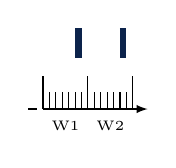
\begin{tikzpicture}[xscale=0.57, baseline={(current bounding box.center)}]
\tikztimeline{2}{7}
\tikztimelineinterval{0+5/7}{0+6/7}{2}{}
\tikztimelineinterval{1+5/7}{1+6/7}{2}{}
\tikztimelineinterval[draw=none,text=black]{0}{1}{-0.5}{\tiny W1}
\tikztimelineinterval[draw=none,text=black]{1}{2}{-0.5}{\tiny W2}
\end{tikzpicture}}}
% Fridays as text
{Fridays}
\right)},
\alt<5->%
% Next(DocTime, January) as timeline
{\text{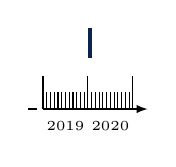
\begin{tikzpicture}[xscale=0.57, baseline={(current bounding box.center)}]
\tikztimeline{2}{12}
\tikztimelineinterval{1+0/12}{1+1/12}{2}{}
\tikztimelineinterval[draw=none,text=black]{0}{1}{-0.5}{\tiny 2019}
\tikztimelineinterval[draw=none,text=black]{1}{2}{-0.5}{\tiny 2020}
\end{tikzpicture}}}
% Next(DocTime, January) as operator
{\operatorname{Next}\left(
\alt<3->%
% DocTime as timeline
{\text{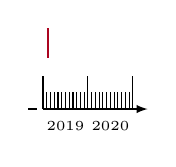
\begin{tikzpicture}[xscale=0.57, baseline={(current bounding box.center)}]
\tikztimeline{2}{12}
\tikztimelineinterval[draw=event]{0+2/24}{0+3/24}{2}{} % bigger than 1/365 to be visible
\tikztimelineinterval[draw=none,text=black]{0}{1}{-0.5}{\tiny 2019}
\tikztimelineinterval[draw=none,text=black]{1}{2}{-0.5}{\tiny 2020}
\end{tikzpicture}}}
% DocTime as operator
{\operatorname{DocTime}},
\alt<3->{%
% January as timeline
\text{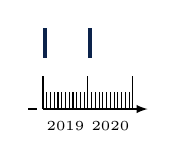
\begin{tikzpicture}[xscale=0.57, baseline={(current bounding box.center)}]
\tikztimeline{2}{12}
\tikztimelineinterval{0+0/12}{0+1/12}{2}{}
\tikztimelineinterval{1+0/12}{1+1/12}{2}{}
\tikztimelineinterval[draw=none,text=black]{0}{1}{-0.5}{\tiny 2019}
\tikztimelineinterval[draw=none,text=black]{1}{2}{-0.5}{\tiny 2020}
\end{tikzpicture}}}
% January as text
{January}
\right)}
\right)}
% Intersection(Union(Mondays, Fridays), Next(DocTime, January)) as text
{}}
$
\end{frame}


\begin{frame}{Machine learning can leverage big data}

\begin{tabular}{ l c c }
\hline\hline
& TempEval 2013 & THYME \\
Model & (News) $F_1$ & (Clinical) $F_1$ \\
\hline
HeidelTime (grammar) & 74 & 70 \\
\AtNextCite{\defcounter{maxnames}{1}}\cite{laparra-etal:2018:TACL} & 77 &  76 \\
\visible<3->{+ FLAIR character representations & 82 & 86} \\
\hline\hline
\end{tabular}

\pause
\bigskip
\AtNextCite{\defcounter{maxnames}{1}}\cite{laparra-etal:2018:TACL} requires manually annotated compositional times for training; only a few thousand exist.

\smallskip
Language models like FLAIR \smallcite{akbik-blythe-vollgraf:2018:C18-1} learn character representations and can train on billions of words of un-annotated text.
\end{frame}


\begin{frame}{Summary}
Deciding how to represent a linguistic phenomenon to a computer is a fundamental challenge in natural language processing

\bigskip
Annotation schemes are representation hypotheses, validated by:
\begin{itemize}
\item agreement between human annotators
\item performance of machine learning models
\end{itemize}

\bigskip
Annotation schemes that decompose complex phenomena yield both better human agreement and better model performance
\end{frame}


\renewcommand{\appendixname}{Supplementary Material}
\appendix


\begin{frame}[allowframebreaks]{References}
\printbibliography
\end{frame}


\end{document}
